\documentclass{ohm_project_description}

\projecttitle{Greifen von Objekten mittels Reinforcement Learning}
\projectauthor{Labor für mobile Robotik}
\projectdate{2025}

\begin{document}

\maketitle
\thispagestyle{fancy}

\vspace*{-2.5cm}
\begin{figure}[h!]
    \centering
    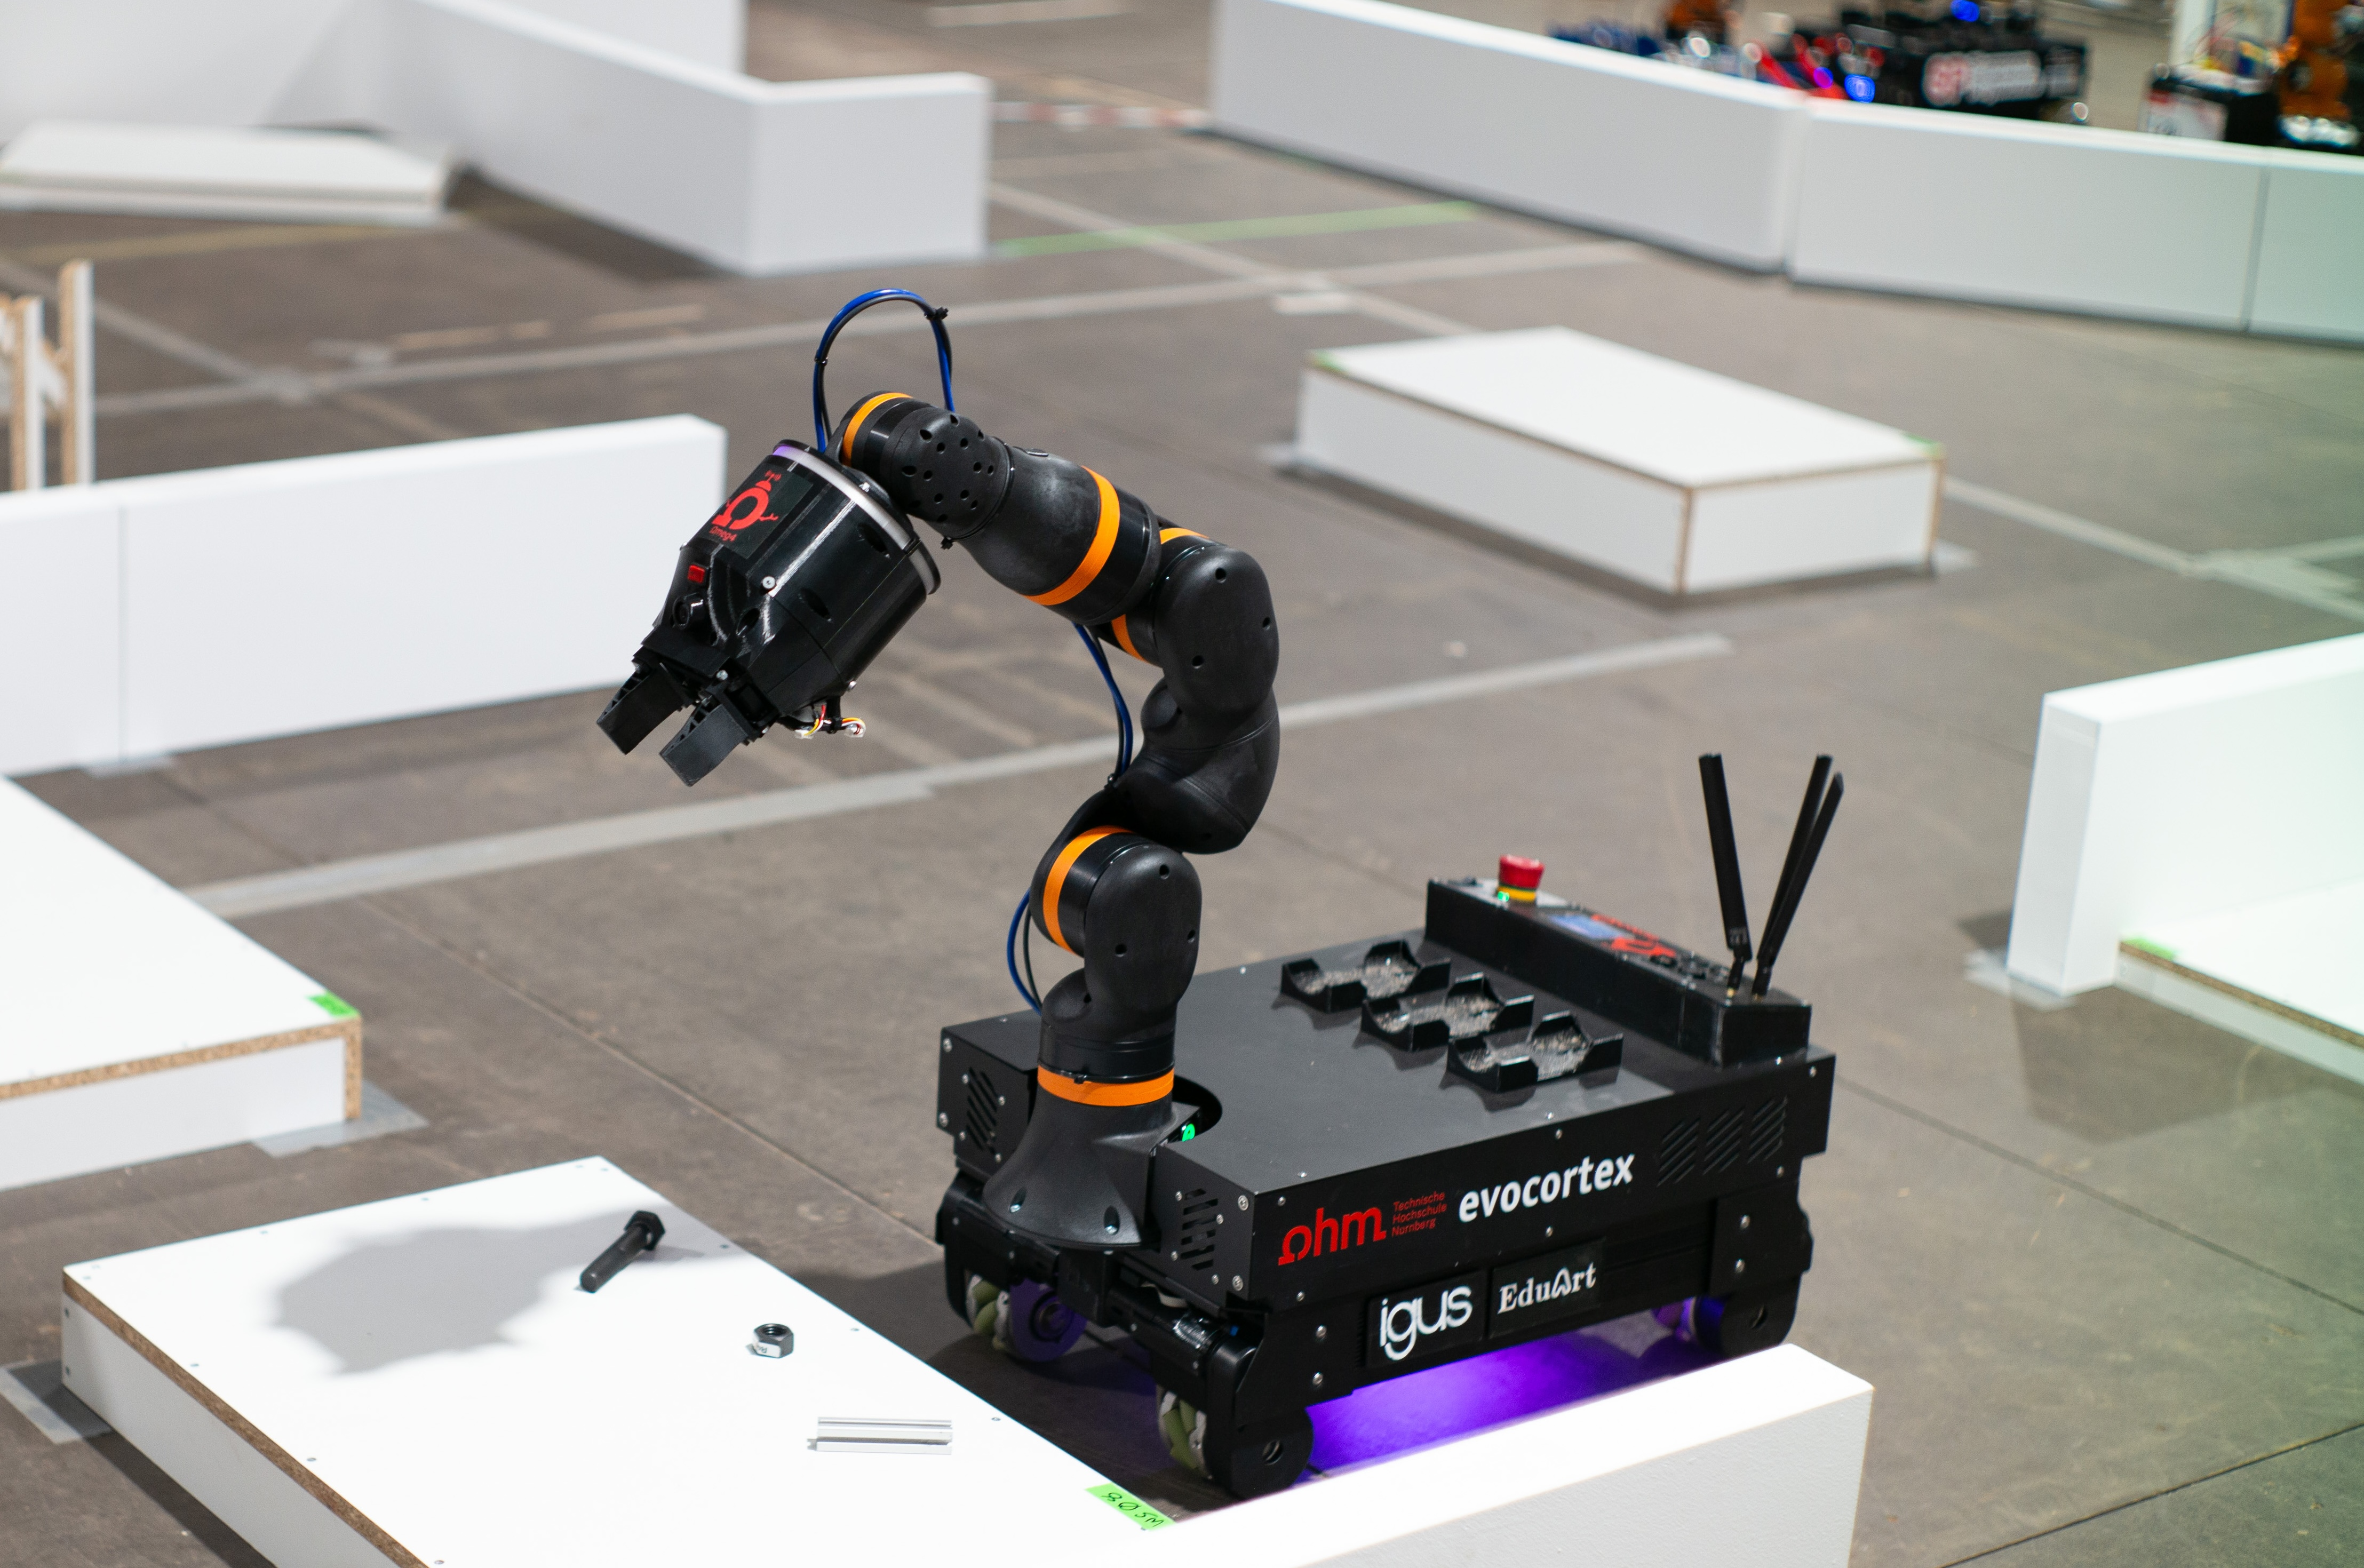
\includegraphics[height=4cm]{img/atwork.jpg}
\end{figure} 


Das Team \textbf{AutonOhm} des Labors für Mobile Robotik nimmt seit vielen Jahren erfolgreich am RoboCup Industrial @Work Wettbewerb teil. Ziel dieses Wettbewerbs ist es, einen mobilen Roboter zu entwickeln, der sich selbstständig in einer Arena zurechtfindet und vordefinierte Aufgaben der Form "Transportiere Gegenstand A von Tisch B zu Tisch C" durchführt. Für diese Aufgaben ist ein komplexes Gesamtsystem aus \emph{Lokalisierung}, \emph{Wahrnehmung}, \emph{Planung} und \emph{Steuerung} notwendig. Es bietet daher für interessierte Studierende neben einer Vielzahl von spannenden Themen im Bereich der mobilen Robotik auch die Möglichkeit, praxisnah an einem \emph{echten} Robotersystem zu arbeiten.

Ein wesentlicher Bestandteil des Systems ist das \emph{Greifen} von Objekten. Aktuell werden die Objekte mittels weniger, vordefinierter Greifposen gegriffen, weshalb ein erfolgreicher Greifvorgang häufig von der Konstruktion des Greiferelements und der Form des Objekts abhängt. Ziel der Arbeit ist es, Reinforcement Learning (bestärkendes Lernen) zu verwernden, um automatisch in Abhängigkeit der Objektform und der Greiferkonstruktion die optimalen Greifpositionen und -bewegungen zu lernen. Dies kann im ersten Schritt in einer Simulationsumgebung erfolgen. Im zweiten Schritt soll das entwickelte Verfahren am echten Roboterarm erprobt werden. 

Engagement und Mitarbeit im studentischen Team Autonohm sind ausdrücklich erwünscht! Es besteht die Möglichkeit, im Rahmen der Arbeit an nationalen und internationalen Wettbewerben teilzunehmen.


\section*{Arbeitspakete}
\begin{itemize}[leftmargin=0.5cm]
    \setlength\itemsep{.1em}
    \item Recherche und Implementierung einer geeigneten Reinformcement-Learning Methode zum optimalen Greifen von verschiedenen starren Objekten
    \item Aufsetzen einer Simulationsumgebung
    \item Training und Validierung der Methode in der Simulation
    \item Training und Validierung an einem echten Roboterarm im Labor
    \item (optional) Integration und Demonstration auf dem mobilen Robotersystem 
\end{itemize}

\section*{Voraussetzungen}
\begin{itemize}[leftmargin=0.5cm]
    \setlength\itemsep{.1em}
    \item Grundkenntnisse in einer höheren Programmiersprache (z.B. Python, C++)
    \item Grundkenntnisse in Deep Learning
    \item (optional) Grundkenntnisse im Bereich Reinforcement Learning
    \item (optional) Grundkenntnisse in ROS
\end{itemize}

\vspace{0.5cm}
Das Thema kann nach Abstimmung als Bachelor- oder Masterarbeit bearbeitet werden, sowie als Projektarbeit. 


\vfill
\textcolor{ohm_red}{\rule{\linewidth}{0.4mm}}
\textbf{\textcolor{ohm_red}{Labor für mobile Robotik}} \\
\begin{tabular}{@{}ll}
\textbf{Betreuer:} & Prof. Dr. Enrico Schröder \\
\textbf{E-Mail:}   & \href{mailto:enrico.schroeder@th-nuernberg.de}{enrico.schroeder@th-nuernberg.de} \\
\end{tabular}

\end{document}